\chapter{Isolierte Ergebnisse}
\label{cha:Isolierte Ergebnisse}


\subsection{reward funktionen}

Previous sections introduced the composite reward function. The composite reward function consists of a weighted sum of individual reward functions. The individual reward functions are designed to encourage the agent to learn the desired behaviour. The goal is to achieve an agent that completes the parcour without collisions, this is encapsulated in the event reward function. However the event reward function is a very spare signal, which makes it hard for the agent to learn. The other individual reward functions are designed to not be sparse, however some of these functions are not enough to guide the agent to the desired behaviour alone, such as the orientation reward.
It is important to find appropriate weights of the individual reward functions for the composite reward function. We are conducting experiments to analyse the usefullness of the individual reward functions. We analyse if the agent is capable of learning the behaviour encouraged by the reward function.

see \ref{table:reward_functions_behaviour}


\begin{table}
    
\caption{Training runs with different reward functions alone (all coefficients 0 except the one of the reward function)}
\begin{center}
\begin{tabular}{|| c | c | c | c ||} 
    \hline
    \makecell{function \\ name} & encouraged behaviour & learned behaviour  & \makecell{expected behaviour \\ learned?} \\ [0.5ex] 
    \hline\hline
    \makecell{event \\ reward} &  \makecell{agent drives through the parcour \\ without collisions} & \makecell{agent turns on the spot \\ continuously} & no \\ 
    \hline
    \makecell{distance \\ reward} & agent drives towards the next goal & agent drives towards the next goal & yes \\
    \hline
    \makecell{orientation \\ reward} & agent turns towards closest goal & \makecell{agent turns around on the spot \\ continuously} & no \\
    \hline
    \makecell{velocity \\ reward}  & full speed ahead (no turning) & full speed ahead (no turning) & yes \\
    \hline
\end{tabular}
\end{center}
\label{table:reward_functions_behaviour}
\end{table}

Note:
it also happened, that the agent turned around and drove backwards (towards the next goal) when given the distance reward only
TODO run these experiments multiple times to see if the results are consistent

--> this shows the distance reward alone might not be the best approach to finding the best policy since it does not encourage driving forward.
--> the agent policy got stuck (turning around and then driving backwards)
    --> from that point the agent cannot conttinue to improve since the agent looks in the wrong direction (important parts are not in field of view)

% TODO
% dieses Verhalten könnte daher kommen, dass die erste Rotation direkt einen hohen distance reward gibt
% die rotation bringt den transform.pos näher zum ersten Tor
% besser wäre es vielleicht den transform.pos eines Punktes/Objekts and der Vorderseite des JetBots zu verwenden


--> distance reward in der derzeitigen Form ist nicht ausreichend
--> im isolierten easy Training lernt er immer mehr reward zu bekommen
--> anstatt ins (letzte) Tor zu fahren dreht er das Hinterteil zum Tor



\subsection{isoliertes Training}



\newcommand{\isolatedImg}[1]{\includegraphics[width=.2\linewidth]{Bilder/isolated/#1}}
\newcommand{\isolatedImgPlaceholder}[1]{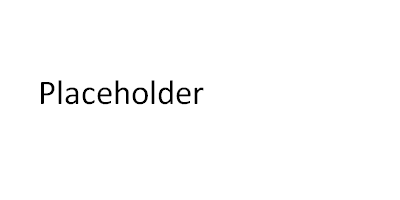
\includegraphics[width=.2\linewidth]{Bilder/isolated/placeholder.png}}

\begin{figure}
\centering
\begin{tabular}{cccc}
          & Easy & Medium & Hard \\
Low  & \isolatedImgPlaceholder{isolated_easy_low_easy_low.png} & \isolatedImgPlaceholder{isolated_medium_low_medium_low.png} & \isolatedImgPlaceholder{isolated_hard_low_hard_low.png} \\
Standard  & \isolatedImg{isolated_easy_standard_easy_standard.png} & \isolatedImg{isolated_medium_standard_medium_standard.png} & \isolatedImg{isolated_hard_standard_hard_standard.png} \\
Bright  & \isolatedImgPlaceholder{isolated_easy_bright_easy_bright.png} & \isolatedImgPlaceholder{isolated_medium_bright_medium_bright.png} & \isolatedImgPlaceholder{isolated_hard_bright_hard_bright.png} 
\end{tabular}
\caption{Figures of isolated training results for their specific setting}
\end{figure}


\subsubsection{light settings}


\newcommand{\esImg}[1]{\includegraphics[width=.2\linewidth]{Bilder/isolated/easy_standard/#1}}
\newcommand{\msImg}[1]{\includegraphics[width=.2\linewidth]{Bilder/isolated/medium_standard/#1}}
\newcommand{\hsImg}[1]{\includegraphics[width=.2\linewidth]{Bilder/isolated/hard_standard/#1}}


\newcommand{\esImgPlaceholder}[1]{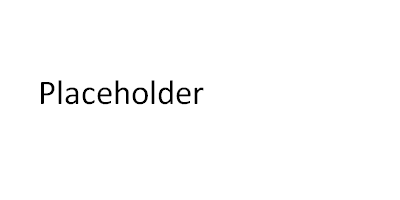
\includegraphics[width=.2\linewidth]{Bilder/isolated/placeholder.png}}
\newcommand{\msImgPlaceholder}[1]{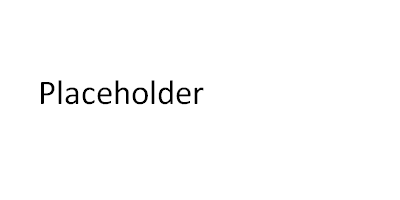
\includegraphics[width=.2\linewidth]{Bilder/isolated/placeholder.png}}


The light setting does not play a significant role in the agent's performance?

\begin{figure}
    \centering
    \esImgPlaceholder{easy_success_rate_comparison.png}
    \caption{easy Difficulty Success Rates for training on easy standard only}
\end{figure}

\begin{figure}
    \centering
    \msImgPlaceholder{medium_success_rate_comparison.png}
    \caption{Medium Difficulty Success Rates for training on medium standard only}
\end{figure}

\begin{figure}
    \centering
    \hsImg{hard_success_rate_comparison.png}
    \caption{Hard Difficulty Success Rates for training on hard standard only}
\end{figure}



\subsection{generalization across difficulty settings}

\begin{figure}
    \centering
    \isolatedImgPlaceholder{easy_tracks_only_all_difficulties_success_rate_comparison.png}
    \isolatedImgPlaceholder{medium_tracks_only_all_difficulties_success_rate_comparison.png}
    \isolatedImg{hard_standard_training-all_difficulties_success_rate_comparison.png}
    \caption{total success rates for difficulties trained on easy, medium and hard only (standard light)}
    \label{fig:isolated_all_difficulties}
\end{figure}

The graph shows that the agents are generally able to generalise to lower difficulty settings \ref{fig:isolated_all_difficulties} .



\subsection{easy standard isolated training}

Agent learned to drive forward through the goals but turn around in front of the last one.
This gives the agent more orientation reward but does not finish the parcour.

see isolated/easy-standard/ gifs

\begin{figure}
    \centering
    \esImg{easy_across_light_settings.PNG}
    \esImg{easy_goal_completion_rate_reward.PNG}
    \esImg{rate_second_given_first.PNG}
    \caption{easy standard}
    \label{fig:isolated_easy_standard}
\end{figure}


